\documentclass[11pt,a4paper]{article}

\usepackage{color,graphicx,listings,wrapfig}
\usepackage[margin=2cm]{geometry}

\graphicspath{{./img/}}

\begin{document}
\title{First report from Threaded Programming}
\author{c02f-32d66e}
\maketitle

\section{Introduction}
The task of this assignment was to pararellise a serial program code downloaded from the \texttt{LEARN} environment. To achieve that we needed to use the OpenMP library and related compiler directives. Because we are more familiar with C than Fortran, C was an obvious choice of language to select for the project. 

As is the case with most parallel programs, the main challenge and focus was not on the speed (which is important), but on being absolutely sure that the program is correct and does not exhibit any erroneous behaviour when scaling to many processors. The given program was fairly simple, so ensuring the correctness was not a hard task, but it nevertheless required careful examination of usage context for every variable.

After ensuring that the program works correctly our task was to see how different choices of schedulers affect its performance. Different considerations put into this part are best described in the corresponding sections later in the report.

\section{Preparation}
\subsection{Code}
Sections that needed paralellisation were identified. There were two loops which work needed to be split among many threads and we decided to use one \texttt{omp parallel for} directive for each loop. We noticed that in both sections it was needed to only make the loop indexes private, as it was never the case that multiple threads attempted to write to the same place in memory in shared arrays. Therefore we did not use critical sections when updating variables inside the loops as they would not yield any benefit for program correctness and would introduce considerable locking overhead. Neither of the loops changes values of non-array variables so they were kept shared to make the memory and communication overhead as low as possible. We also decided that we will not use the \texttt{default(none)} clause, even though it has some educational use, as using clear implicit rules that save typing is a good foundation of a sound programming practice.

The Unix \texttt{sed} program was used for generating versions of the source code with different schedulers and chunks sizes. Its output was then fed to \texttt{gcc} and compiled with the \texttt{-O3} code optimisation level. Each of the cases to be tested was then executed ten times on \texttt{Morar} using the \texttt{qsub} utility. We decided that executing each of the cases ten times strikes at a balance between the accuracy of determining the time variability for each run and making the usage of the machine inconvenient for other users.

\subsection{Data methodology}
We were not sure at first if we should use the fastest time for each case as its result, or take the average of the runs and use the standard deviation as a measure of time variability. The first method has a marked advantage, as all of the slower than fastest runs are caused by another processes using the machine. On the other hand the potential user is usually interested in `real life' runs of the program and as such a program that is strongly influenced by other programs running alongside it will not be the most useful one, even if it is faster than all the others in the most optimal case. 

Because of that we decided to report the average time for each test case. As it turned out, the standard deviation for all the measurement points was smaller than the point size on the graph, so at the end we decided not to plot it, to keep the plots clear and readable.

\section{Results}
\subsection{Choosing the fastest scheduler}
\subsubsection{First loop}
At first the parallel version of the code was run with different schedulers and different chunk sizes (when applicable). Each of the runs was repeated ten times to estimate the runtime variability which, as mentioned, turned out to be minimal. As can be seen on Figure~\ref{loop1} different schedulers produce markedly different results, but for the first loop either the \texttt{static} scheduler with chunk size \(\leq 8\) could be used or \texttt{dynamic} with chunk size \(\leq 16\). The times for both \texttt{auto} and \texttt{static} were too long to be considered in the speed contest for the first loop.

\begin{figure}[h!]
    \begin{center}
        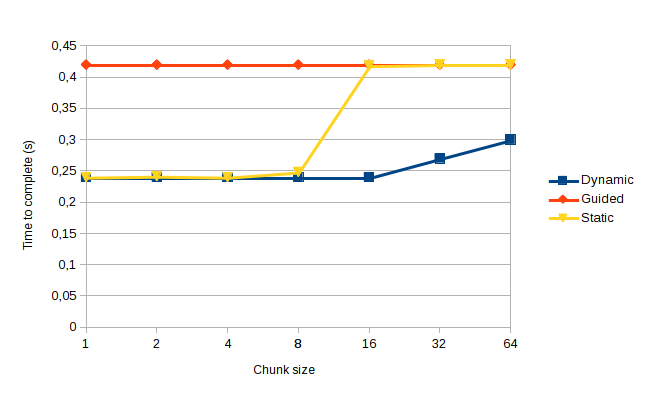
\includegraphics[width=0.8\textwidth]{loop1.png}
    \end{center}
    \caption{Run times for different schedulers and chunk sizes for the loop 1. The two schedulers without a specified chunk size, \texttt{auto} and \texttt{static} (with no parameter specified) both ran in \(0.41s\).}
    \label{loop1}
\end{figure}

Looking at the code of the first loop reveals the sources of behaviour under different schedulers. The loop has most of its work at its beginning, which explains the constant time achieved with the \texttt{dynamic} scheduler and different chunk sizes. It also explains why the \texttt{static} scheduler is working fast with small chunk sizes, but starts to lag behind \texttt{dynamic} for larger ones - as the chunk size grows larger the amount of work in different threads gets more and more unbalanced, thus leading to the threads with less work to wait for the threads which had more work assigned to them. The \texttt{dynamic} scheduler wins for every chunk size, as the flexibility arising from each thread being able to pick up the next outstanding chunk apparently outweighs the communication costs.

\subsubsection{Second loop}
\label{second}
The results obtained for the second loop were much more varied. We can again readily notice the constant time for the \texttt{guided} scheduler, but there is a strong time minimum for both \texttt{static} and \texttt{dynamic} schedulers.

If we look carefully at how the number of iterations is assigned to the loop with iterator \textit{j}, we notice that when \textit{i} is less than 30, \textit{j} is bounded by \(0 \leq j < N\). When \(30 \leq i < 60\), only one in four \textit{j}s is assigned N iterations and the rest gets only one. In the following 30 only one in seven and so on (see line 73 in \texttt{loops.c})\footnote{The innermost loop with index \textit{k} does the same number of iterations as the loop indexed by \textit{j} does. Therefore any influence the \textit{j} range has is quadratic!}. Therefore the bulk of the computations is again at the beginning of the outermost loop, which explains the consistent behaviour of the \texttt{guided} scheduler. The number of computations is even more skewed towards the beginning of the \textit{i} loop than it seems at the first sight, as the total number of \textit{i} for which \textit{j} does more than one iteration is only 67\footnote{This was determined by a simple one-line Python script implementing the condition from line 73.}.

\begin{figure}[h!]
    \begin{center}
        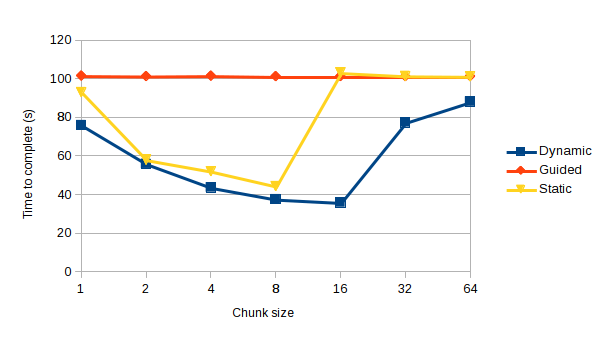
\includegraphics[width=0.8\textwidth]{loop2.png}
    \end{center}
    \caption{Run times for different schedulers and chunk sizes for the loop 2. For the \texttt{auto} and \texttt{static} schedulers, without chunk size specified, we observe the execution times of \(99s\) and \(100s\) respectively.}
\end{figure}

Since the workload change period is 30, we would expect the most efficient scheduler to be the one with a chunk size as close to 30 as possible, but that is not what happens. Instead we observe the time for both \texttt{static} and \texttt{dynamic} schedulers to decrease at first, but then drastically increase after the chunk size of 8 and 16 (respectively) is passed. For both schedulers the time taken decreases at first, as increasing the chunk size decreases the overhead due to switching between the chunks. Above the chunk size of 8, the \texttt{static} scheduler speed decreases drastically as imbalance in the number of computations in different threads increases - in the case of the chunk size of 32, the first thread has half of the workload of the whole \textit{i} loop!

Due to its higher complexity the behaviour of the \texttt{dynamic} scheduler is less simple. The decrease in the time taken to complete the loop at the chunk sizes \(\leq 16\) is due to decreasing chunk switching overhead. The time increase for chunk sizes higher than 16 can only be explained if we remind ourself that the total number of \textit{i} for which the \textit{j} loop needs to do more than one iteration is 67. As \(67 / 4= 16.75 \) and the bulk of computational load is in those iterations of the outer loop when \textit{j} does N iterations we see that at higher chunk sizes than 16 it is impossible to distribute the computational load among the threads evenly. The influence of this uneven distribution gets bigger as the chunk size increases.

\subsection{Choice of the scheduler}
It is clear that the second loop performs best with the \texttt{dynamic} scheduler, and chunk size of 16. The picture is much more uncertain for the first loop, though. Should we use the \texttt{static} or \texttt{dynamic}, if so with what chunk size? We have decided that it would be better to make both loops use the same scheduler and chunk size, if possible. Such a choice makes the program more convergent and if there is no performance penalty in doing so, it is the right choice to make from software development perspective.

As can be seen on both plots, \texttt{dynamic} scheduler with the chunk size of 16 is the most efficient one for both loops, so it was chosen in both cases.

\subsection{Measuring parallel speedup}
The parallel speedup is presented on Figure~\ref{speedup}. The striking feature of the graph is the visibly different scaling properties for the first and the second loops. 

\begin{figure}[h!]
    \begin{center}
        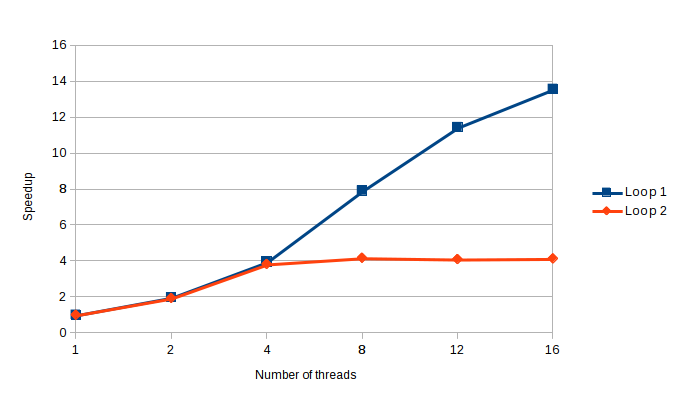
\includegraphics[width=0.8\textwidth]{speedup.png}
    \end{center}
    \caption{Speedup for both loops ran with different number of threads. The speedup is defined as \(T_1 / T_p\), where \(T_1\) is the execution time on one processor and \(T_p\) on \textit{p} processors.}
    \label{speedup}
\end{figure}

To understand why the second loop performance plateaus at the number of processors \( > 4\), we need to remind ourselves of the amount of work that the program needs to do in the second loop. There are only 67 iterations that carry significant computational load (as explained in Section~\ref{second}). Therefore when using the chunk size of 16 there will be at most four cores doing significant work\footnote{Because the \texttt{dynamic} scheduler assigns the next work chunk on `first come, first served' basis, more than four cores will do work during the course of the program execution. However, the number of cores doing any significant work at any given moment will be equivalent to four cores.} at any given time. We observe this effect on the speedup graph, with the slight difference between 8 and 4 cores arising from having spare computing power to deal with the low-load iterations.

The first loop scales well until the number of threads reaches 16, at which point the fact that each thread will on average do only 3 chunk switches takes its toll. It is because with a chunk size of 16 and 16 threads, we get \(16 * 16 = 256\) iterations assigned to different threads at the start. Because the amount of computations decreases as the loop progresses, the high-numbered threads will need to change chunks more frequently than the low-numbered ones, thus making the communication overhead impose a performance penalty.

\section{Conclusions}
As the test data shows, the choice of a scheduler and chunk size is an important factor in the performance of parallel loops. The best performing scheduler and chunk size on four threads need not be the most optimal choice on higher (or lower) number of threads. In fact, we predict that higher performance for the second loop on more than four threads could be achieved by lowering the chunk size to eight or even four. Additional investigation in the effect of lowering the chunk size is warranted. Further performance gains may be achieved by using different compilers, but this is outside of scope for this report. 

The results show importance of understanding the nature of calculations that the parallel code is doing to achieve an optimal execution performance. Such an insight is harder to achieve as the code complexity grows, at which point the experimental tests presented in the report gain importance. Regardless of the code complexity, for a well designed program it should be possible to combine the understanding of computations the code is doing with experimental data to ensure optimal code performance on different computer systems.


\end{document}
